\chapter*{タイルマップサービス(TMS)とは}

GoogleMapsのように、表示する位置や縮尺を自由に変えられる地図をslippy mapといいます。
日本語では「スクロール地図」でしょうか。
さて、このslippy mapを作って欲しいと依頼された時、あなたはどのように実装しますか?

まず地図の情報が必要です。それは画像である必要があります。
その画像を切り出してブラウザに表示する...ざっくりそんな感じになるでしょうか。
まさにこれを実装したのが、タイルマップサービス(Tile Map Service) TMSと
よばれるものです。
%
TMSは、正確に言うと Open Source Geospatial Fundation (OSGeo財団)によって開発された
タイルの仕様で、オープンソースなプロダクトによく使われています。
同様の機能を実現した、WMTS (Web Map Tile Service)というものもあります。

\subsection*{タイル}
一枚の大きな世界地図を、小片に分割して必要なものだけ送ることで、ネットワークの帯域やメモリの消費を抑えることができます。
この分割された地図の小片を「タイル」と呼びます。
TMSでは、タイルは一辺が256ピクセルの正方形のPNG画像です。
次にタイルの切り出し方を考えます。
まず、世界地図を1枚のタイルで表現することができます。この縮尺をズームレベル0と呼びます。
ズームレベルは、正の整数値で、1増える毎に表示する面積が1/4になります。
すなわち、ズームレベル1では、縦2枚、横2枚の4枚のタイルで全世界を表現します。
同様にズームレベル2では、16枚になります。
これを繰り返していくと、図\ref{fig:tile_pylamid}のようなピラミッド構造になります。

\begin{figure}[thbp]
\centering
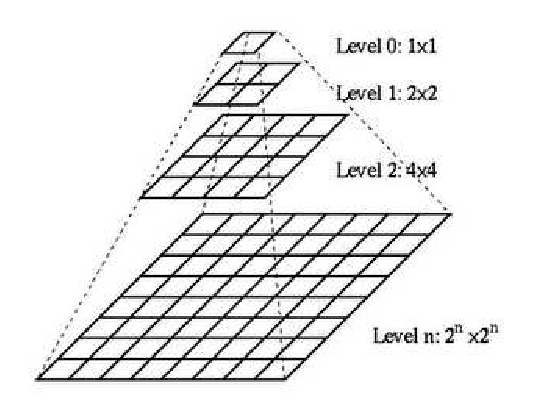
\includegraphics{Tiling.eps}
\caption{タイルのピラミッド構造\cite{ref:tile}}
\label{fig:tile_pylamid}
\end{figure}

このタイルの位置は、x、yの座標で、OpenStreetMapでは、緯度経度との関係は以下の通りです。
\[
x = \frac{2^z(lon+180)}{360}
\]
\[
y = 2^{z-1}(1-\frac{\ln(\tan(\frac{lat\pi}{180})+\sec(\frac{lat\pi}{180}))}{\pi})
\]
ここで、$lon$、$lat$は、それぞれ度単位の経度、緯度、$z$はズームレベルです。
ちなみにxyの原点は...って聞かれると、
TMSは左下で、WMTSは右上で、OpenStreetMapは、Y flipped TMSとやらで、左上だったり、
結構闇だったりします。上の式はOpenStreetMapのものなので、TMSとは異なるので注意が必要です。

\subsection*{タイルの配布}
さて、タイルのことはわかってきました。それでは、どのようにタイルを取得するすれば良いのでしょう。
TMSはブラウザに地図を表示するためのものですので、もちろんWebサーバからHTTPで取得します。
URLは、以下のようになります。
\begin{center}
  \texttt{http://tms.example.org/1.0.0/name/z/x/y.png}
\end{center}

x、yはタイルの座標で、zはズームレベル、1.0.0というのはTMSのバージョンです。
nameはタイルの名前です。
例えば、地理院地図の50万分の1のタイルのURLは
\begin{center}
  \texttt{http://cyberjapandata.gsi.go.jp/xyz/std/z/x/y.png}
\end{center}
となります。
実際のタイルサーバでは、TMSのバージョンがなかったり、結構自由です。
正確には地理院地図はTMSと名乗っていません。
ただ、TMSもWMTSも地理院地図もOpenStreetMapも、URLでXYZを指定してタイルを取得するので
これらを総称してXYZタイルやXYZレイヤなどと呼ばれています。
仕様はがっちり決められていても、実装が追いつかないのはよくある話ですね。

この本でも、がっちりTMSを実装するのではなく、ざっくりXYZタイルサービスを作成することにしましょう。

\subsection*{タイルの作成}
では、タイルを作成しましょう。
元になる、測地系といった地理空間情報が付いた画像があれば簡単です。
例えば、world.tiffという、GeoTiffファイルがあったとしましょう。
GeoTiffファイルは、地理空間情報のタグが付加されたTiff画像です。
地理空間情報が付いたフォーマットにShape等もありますが、21世紀なのでGeoTiffで良いでしょう。
タイルの作成には、GDALに入っているgdal2tiles.pyを使います。
GDALは、''ぐーだる''とか''ぐだーる''と呼ばれている、Geoな世界のスイスアーミーナイフ的な
存在で、本来はC/C++のライブラリなのですが、付属するプログラムが優秀でツール群と誤解されているものです。
後で、プログラミングライブラリとして使用しますが、タイルの生成には、GDALをツール群として使います。GDALのインストールは面倒なイメージがあるので、LinuxのパッケージやOSGeoLiveといったディストロを使うと良いでしょう。
特にOSGeoLiveはGeoな事をやる時に必要なツールはほとんど入っているので、特におすすめです。

タイルの作り方ですが、gdal2tiles.pyにGeoTiffファイル名を指定するだけです。
生成するタイルのズームレベルの範囲を指定することもできます。
たとえば、map.tiffから、ズームレベル0から8までのタイルを生成するには、以下のコマンドを実行します。

%\begin{center}
\texttt{\$ gdal2tiles.py -z 0-8 map.tiff}
%\end{center}

タイルの生成には、大量の画像を生成するためものすごーく時間がかかります。
ちなみにズームレベル0から8までのタイルの総数は87,381枚です。

さて次章では、タイルを生成する元ととなる、GeoTiffファイルを作成します。
